\section{Syntax representation}\label{sec:syntaxrepr}
% \sideboxbegin{o}
% This section presents the limitation encountered while integrating the functionalities of Trace\textit{a} into SysMLv2.
% \sideboxend

In this section we present the different means a user can take a trace to work with. The first version shows a key representation based on Traces's metamodel properties expressed in JSon. The second version is slightly augmented to allow its visualization using the D3-JS API\footnote{\url{https://d3js.org/}}. Last but not least, a matrix-based representation facilitates the analysis of a trace and gives a useful HTML visualization.

\subsection{Trace\textit{a} model}
\label{sec:traceamodel}
\begin{figure}[ht]
	\centering
	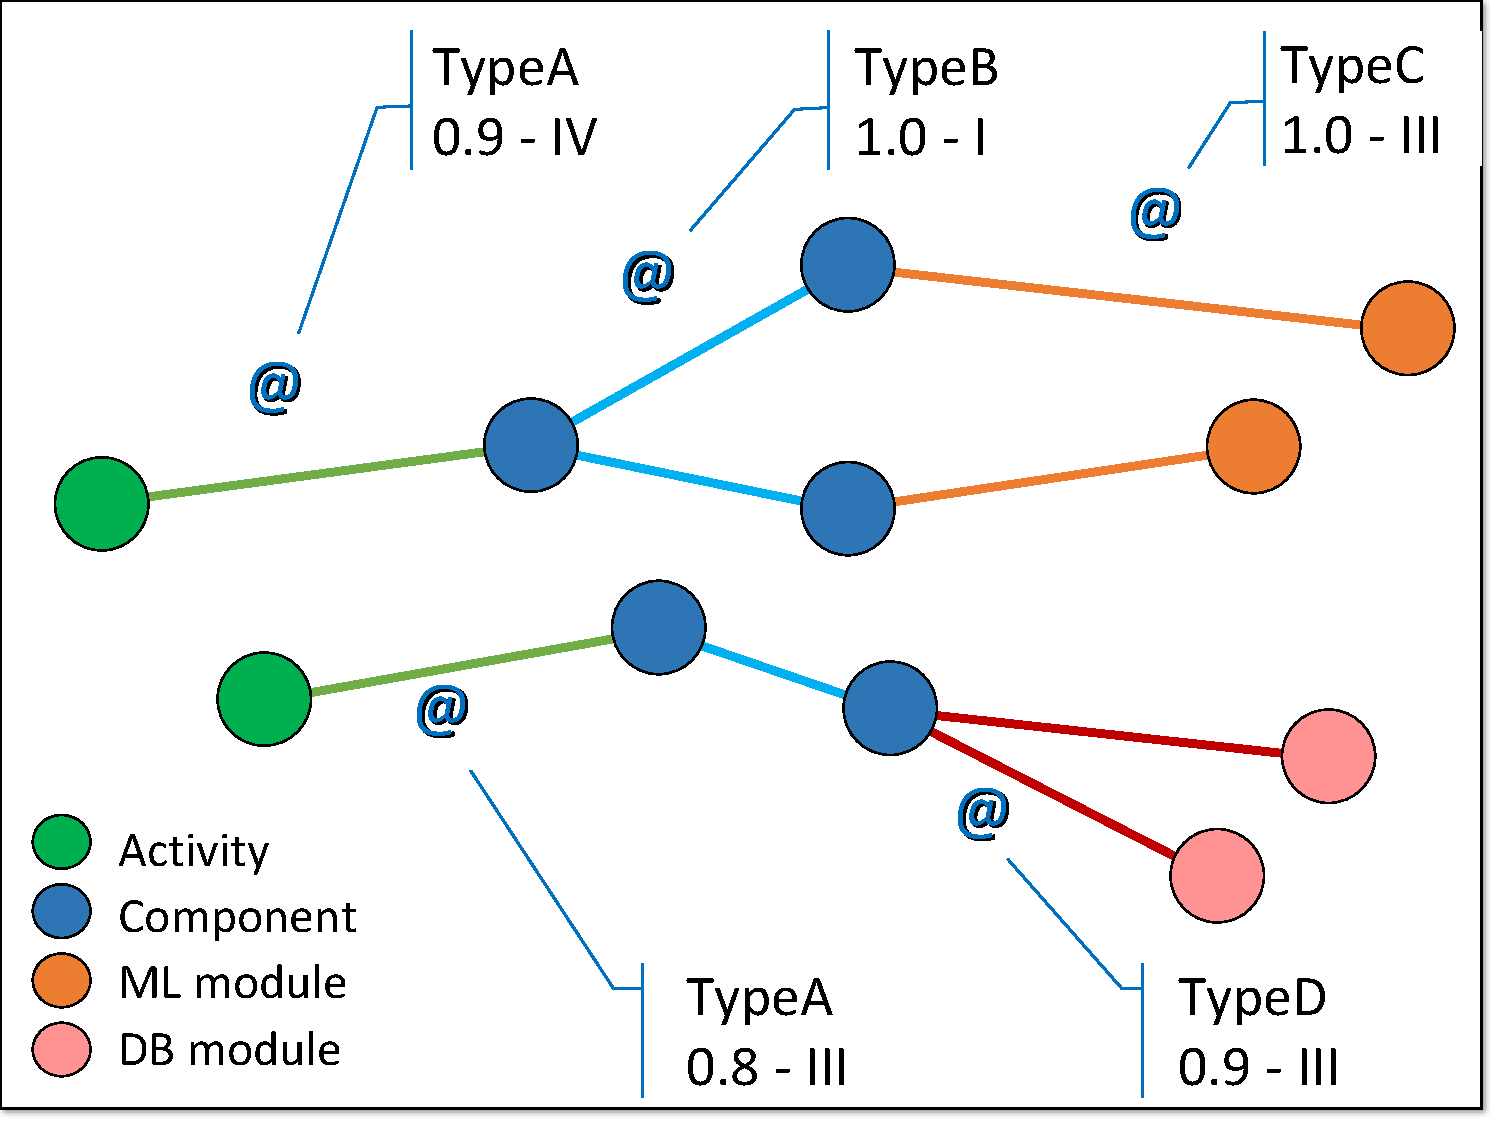
\includegraphics[width=.5\linewidth]{images/energy3.pdf}
	\caption{An illustrative example of a Tracea model.}
	\label{fig:traceamodel}
\end{figure} 
The first representation reflects directly the complex nature of the trace using Trace\textit{a}-like representation. Links are encoded with multiple types and can be multi-ended (source and target alike). This raw representation is the working base for future transformation into specific visualizations, characterized representations, or further mathematical analysis. An illustrative example of a Tracea model is given in \Fig{fig:traceamodel}. Its textual representation is shown in the excerpt of Listing~\ref{lst:traceamodel}.

\begin{center}
\begin{lstlisting}[caption={Excerpt of a trace written in Tracea-JSon.},
label=lst:traceamodel,
style=mystylesysml,
frame=shadowbox,
rulesepcolor=\color{blue},
linewidth=16.6cm,
xleftmargin=0.2cm,
morekeywords={links,id,name,type, source_id, target_id,confidence,nodes,qualifiedName,types,sources,targets}]
{
 "links": [
  { 
    "id": "1085", 
    "name": "eng2front", 
    "qualifiedName": "eDrone_example::eng2front", 
    "types": ["TypeE"], 
    "sources": [{ "id": "b9bb"}],
    "targets": [{ "id": "3adb"}], 
    "confidence": 0.85
  }
   /* ... */
 ], "nodes": [
  { 
    "id": "d83f", 
    "name": "eDrone.battery", 
    "type": "Feature"
  }
  /* ... */
]
}
\end{lstlisting}
\end{center}

\subsection{SysML reinjection}
The Tracea model allows the generation of SysML code to reinject modification, or to populate a model from sources external from the target languages (here SYsML). Listing~\ref{lst:sysmlout} shows a (modified) trace that can be reinjected in the original the model as depicted earlier in \Fig{fig:reinject}.
\begin{center}
\begin{lstlisting}[caption={SysML code generated from a Tracea model.},
label=lst:sysmlout,
style=mystylesysml,
frame=shadowbox,
rulesepcolor=\color{blue},
linewidth=16.6cm,
xleftmargin=0.2cm,
morekeywords={connection,connect,to,metadata,about}]
/* Trace links */
connection eng2front connect eDrone.engine to eDrone.frontAxis;
connection frAx2frWi connect eDrone.frontAxis to eDrone.frontWing;
connection reAx2reWi connect eDrone.rearAxis to eDrone.rearWing;
connection bod2bat connect eDrone.body to eDrone.battery;
connection bod2eng connect eDrone.body to eDrone.engine;
connection bod2frAx connect eDrone.body to eDrone.frontAxis;
connection bod2reAx connect eDrone.body to eDrone.rearAxis;
connection eng2bat_Typed connect eDrone.battery.powerOut to eDrone.engine.powerIn;
connection rq1ToWing connect eDroneMaxSpeed to eDrone.engine;
connection refine1 connect eDrone.battery to eDrone.battery.powerOut;
connection refine2 connect eDrone.battery to eDrone.engine.powerIn;

/* Tracing metadata */
metadata m6093: ConfidenceTracing about eng2front { confidence = 0.85;}
metadata m4103: TraceType about eng2front { tracetype = "TypeE";}
metadata m5096: ConfidenceTracing about frAx2frWi { confidence = 0.65;}
metadata m9040: TraceType about frAx2frWi { tracetype = "TypeE";}
metadata m7556: ConfidenceTracing about reAx2reWi { confidence = 0.75;}
metadata m9270: TraceType about reAx2reWi { tracetype = "TypeE";}
metadata m8202: TraceType about bod2bat { tracetype = "Internal";}
metadata m9711: TraceType about bod2eng { tracetype = "Internal";}
metadata m8159: TraceType about bod2frAx { tracetype = "Internal";}
metadata m7086: TraceType about bod2reAx { tracetype = "Internal";}
metadata m7259: ConfidenceTracing about eng2bat_Typed { confidence = 0.65;}
metadata m3388: TraceType about eng2bat_Typed { tracetype = "TypeA";}
metadata m9094: ConfidenceTracing about rq1ToWing { confidence = 0.45;}
metadata m5621: TraceType about rq1ToWing { tracetype = "TypeA";}
metadata m340: ConfidenceTracing about refine1 { confidence = 0.45;}
metadata m8719: TraceType about refine1 { tracetype = "Convenience";}
metadata m5065: ConfidenceTracing about refine2 { confidence = 0.55;}
metadata m8879: TraceType about refine2 { tracetype = "Convenience";}
\end{lstlisting}
\end{center}

\subsection{Graph visualization}
The literature mention extensively the need for higher level representation to apprehend the inherent complexity of traces. In the end of the day, they are graphs and it sounds of utmost importance to represent them graphically. \Fig{fig:visualizationgraph} shows a graph-based representation of a trace. Each link is an edges between two node-elements. Here, representing multi-ended links is arduous and would require strong decisions. The multi-typed nature of links would need also a further investigation to decide whether to decide the types to show beforehand, or to allow a more interactive manipulation in which there is options to allow users to change them on the fly.

\ugh{Interactivity: confidence/cost thresholds ; tickers for types ; ...}

\begin{figure}[h]
	\centering
	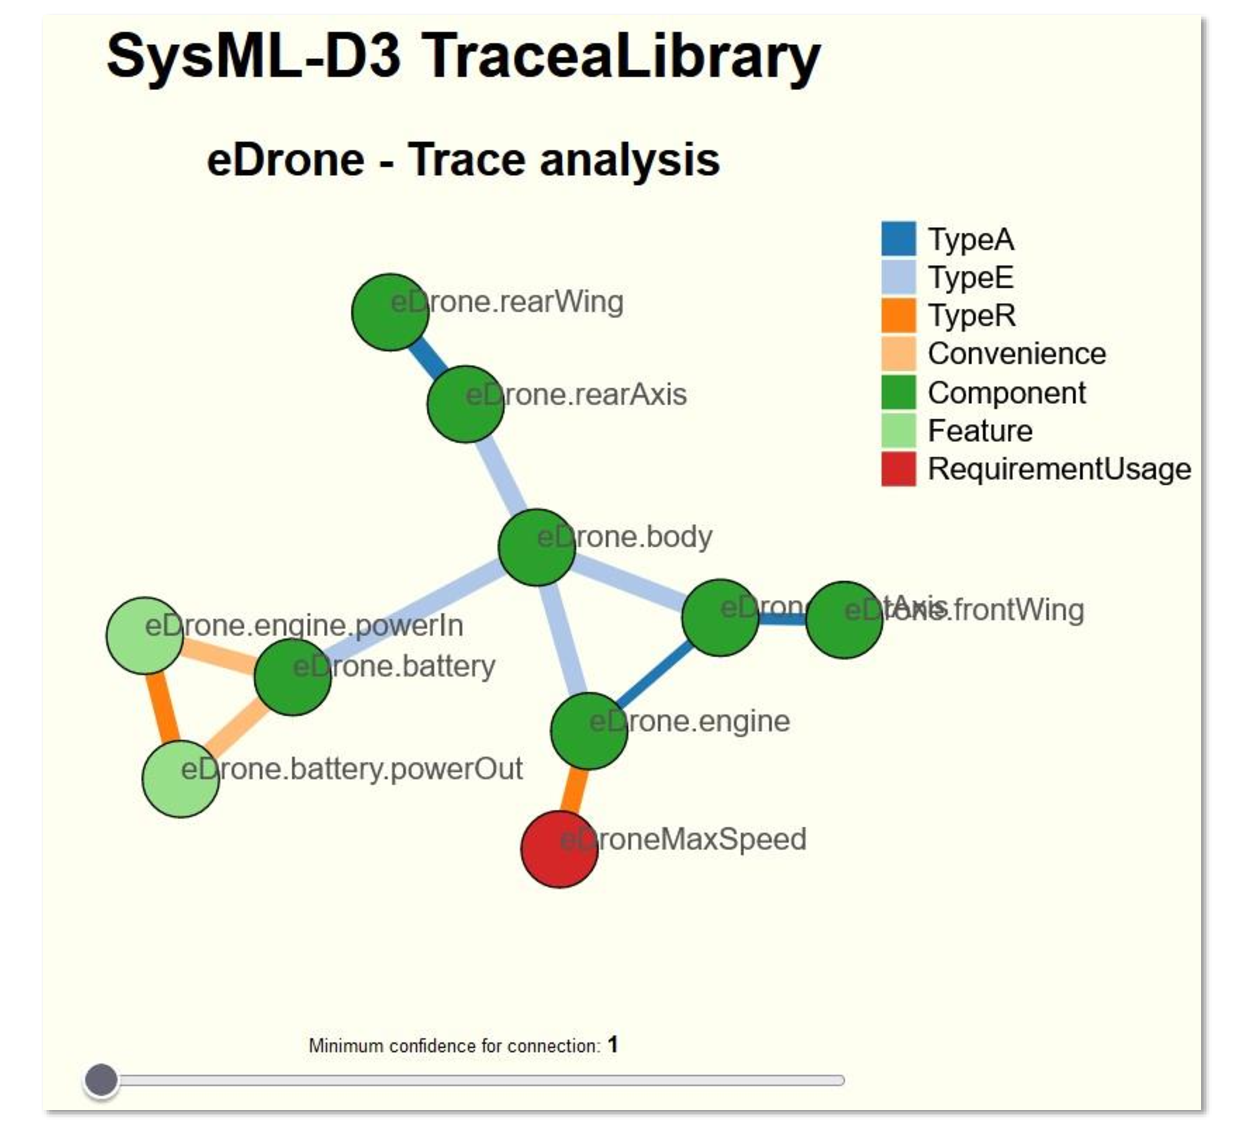
\includegraphics[width=.6\linewidth]{images/visualization1.pdf}
	\caption{A graph-based visualization of a Trace.} 
	\label{fig:visualizationgraph}
\end{figure}

\subsection{Matrix-based view}
Finally, we offer the alternative matrix-based representation of the traces. We export the Trace\textit{a model} as text and HTML tables. The latter is rather interesting. The use of interactive instances of HTML in conjunct use with CSS-JS will allow a valuable set of tools to explore the trace.

\begin{figure}[h]
	\centering
	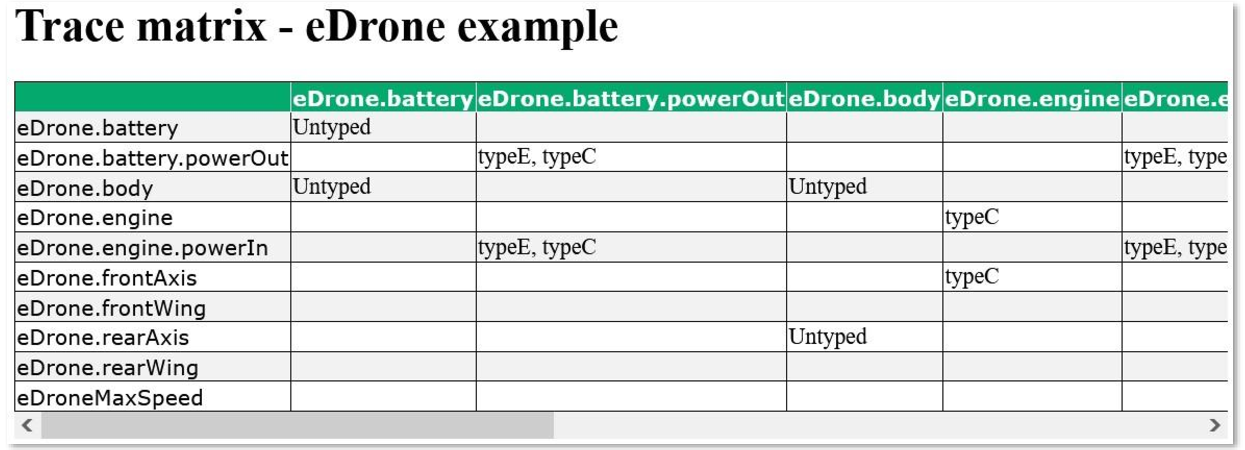
\includegraphics[width=.85\linewidth]{images/matrix1.pdf}
	\caption{A matrix-based representation of a Trace.}
	\label{fig:matrixview}
\end{figure}

\subsection{Interactive features planned}
Using an external tool to handle traces then serves to populate the trace from external sources. In this fashion, an interactive UI shall offer:
\begin{itemize}
    \item To assign trace types to links and define which ones are shown (tickers)
    \item To identify and target ends for links (potentially from a base of tagged elements ?)
    \item To show metadata features (parametered on demand)
    \item To filter links based on thresholds: confidence, cost, energy consumption; or on their type, name, end types...
    \item To export result after manipulation: results of the selection of links / elements, and to export the edited links.
\end{itemize}
 
